% Shared standalone design for the editable figure reconstructions.
\documentclass[tikz,border=5pt,10pt]{standalone}
\usepackage[T1]{fontenc}
\usepackage[utf8]{inputenc}
\usepackage{newpxtext,newpxmath}
\usepackage[scaled=.94]{sourcesanspro}
\usepackage{pgfplots}
\pgfplotsset{compat=1.18}
\usetikzlibrary{arrows.meta,calc,positioning,decorations.pathreplacing,
  decorations.markings,patterns,matrix,shapes.geometric,fit,backgrounds,
  intersections,angles,quotes}
\definecolor{ink}{HTML}{203746}
\definecolor{accent}{HTML}{146C78}
\definecolor{muted}{HTML}{667780}
\definecolor{signalred}{HTML}{B94B44}
\color{ink}
\tikzset{>=Latex,line width=.8pt,
  every node/.style={font=\small},
  axis/.style={->,draw=muted,line width=.5pt},
  guide/.style={draw=muted,dashed,line width=.45pt},
  curve/.style={draw=accent,line width=1pt},
  marker/.style={circle,fill=accent,inner sep=1.5pt},
  labelbox/.style={fill=white,inner sep=2pt}}

\begin{document}
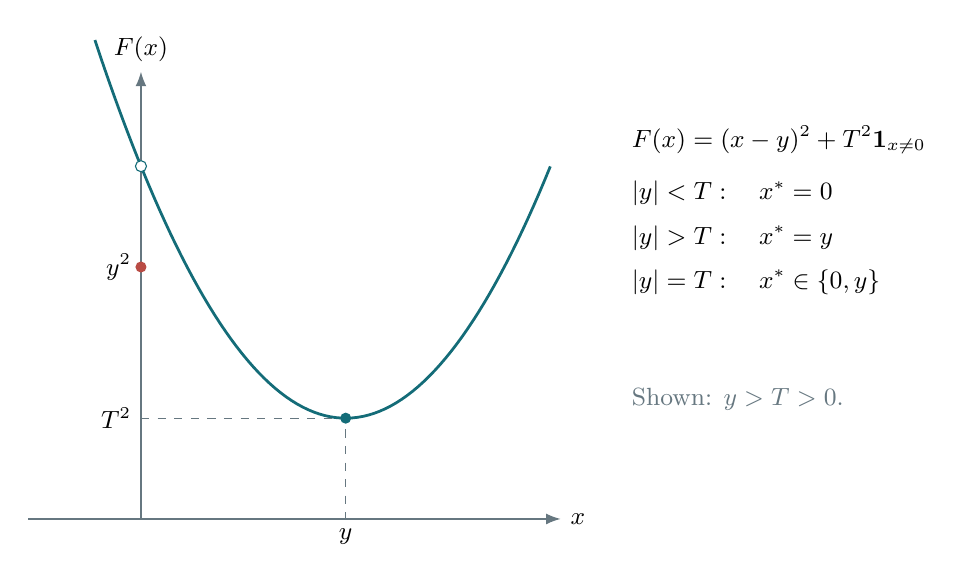
\begin{tikzpicture}[x=1.3cm,y=.8cm]
\draw[axis](-1.1,0)--(4.1,0)node[right]{$x$};\draw[axis](0,0)--(0,7.1)node[above]{$F(x)$};
\draw[curve]plot[domain=-.45:-.02,samples=30](\x,{(\x-2)^2+1.6});
\draw[curve]plot[domain=.02:4,samples=75](\x,{(\x-2)^2+1.6});
\filldraw[draw=accent,fill=white](0,5.6)circle(2pt);
\fill[signalred](0,4)circle(2pt);\node[left]at(0,4){$y^2$};
\draw[guide](0,1.6)node[left]{$T^2$}--(2,1.6)--(2,0)node[below]{$y$};\fill[accent](2,1.6)circle(2pt);
\node[anchor=west,align=left]at(4.7,4.9){$F(x)=(x-y)^2+T^2\mathbf1_{x\ne0}$\\[8pt]$|y|<T:\quad x^*=0$\\[5pt]$|y|>T:\quad x^*=y$\\[5pt]$|y|=T:\quad x^*\in\{0,y\}$};
\node[muted,anchor=west]at(4.7,1.9){Shown: $y>T>0$.};
\end{tikzpicture}
\end{document}
